%%%%%%%%%%%%%%%%%%%%%%%%%%%%%%%%%%%%%%%%%
% University/School Laboratory Report
% LaTeX Template
% Version 3.1 (25/3/14)
%
% This template has been downloaded from:
% http://www.LaTeXTemplates.com
%
% Original author:
% Linux and Unix Users Group at Virginia Tech Wiki 
% (https://vtluug.org/wiki/Example_LaTeX_chem_lab_report)
%
% License:
% CC BY-NC-SA 3.0 (http://creativecommons.org/licenses/by-nc-sa/3.0/)
%
%%%%%%%%%%%%%%%%%%%%%%%%%%%%%%%%%%%%%%%%%

%----------------------------------------------------------------------------------------
%	PACKAGES AND DOCUMENT CONFIGURATIONS
%----------------------------------------------------------------------------------------

\documentclass{article}

\usepackage[version=3]{mhchem} % Package for chemical equation typesetting
\usepackage{siunitx} % Provides the \SI{}{} and \si{} command for typesetting SI units
\usepackage{graphicx} % Required for the inclusion of images
\usepackage{natbib} % Required to change bibliography style to APA
\usepackage{amsmath} % Required for some math elements 
\usepackage[utf8]{inputenc}
\usepackage[margin=1.2in]{geometry}

\setlength\parindent{0pt} % Removes all indentation from paragraphs

% \renewcommand{\labelenumi}{\alph{enumi}.} % Make numbering in the enumerate environment by letter rather than number (e.g. section 6)

\renewcommand{\figurename}{Figura}
\renewcommand{\tablename}{Tabla}
\renewcommand\refname{Referencias}

\def\mean#1{\left< #1 \right>}
%\usepackage{times} % Uncomment to use the Times New Roman font

%----------------------------------------------------------------------------------------
%	DOCUMENT INFORMATION
%----------------------------------------------------------------------------------------

\title{M\'etodos num\'ericos para la Ciencia e Ingenier\'ia \\ Tarea 6: Métodos Aleatorios} % Title

\author{Felipe Toledo Bittner} % Author name

\date{\today} % Date for the report

\begin{document}

\maketitle % Insert the title, author and date

%----------------------------------------------------------------------------------------
%	SECTION 1
%----------------------------------------------------------------------------------------

\section{Integración de Montecarlo}

\subsection{Introducción}
\label{sec:introduccion_P1}

Se desea obtener la posición del centro de masa de un sólido formado por la intersección de un toro con un cilindro, descrito por las ecuaciones (\ref{eq:toro}) y (\ref{eq:cilindro}).

\begin{equation}
  Toro:\ z^2 + \left( \sqrt{x^2 + y^2} - 3 \right)^2 \leq 1
  \label{eq:toro}
\end{equation}

\begin{equation}
  Cilindro:\ (x - 2)^2 + z^2 \leq 1
  \label{eq:cilindro}
\end{equation}

La densidad del sólido no es uniforme y es descrita por la fórmula (\ref{eq:densidad}). Debido a esto último, realizar una integración analítica para encontrar el centro de masa puede resultar complejo, por lo que se decide utilizar el método numérico de Monte Carlo para estimar su posición.

\begin{equation}
  \rho(x, y, z) = 0.5 (x^2 + y^2 + z^2)
  \label{eq:densidad}
\end{equation}

Las integrales que se deben calcular para obtener la coordenada $x^i$ del centro de masa son las siguientes:

\begin{equation}
  M = \int_V \rho(\vec{r}) dx dy dz \approx \sum_j \rho(\vec{r_j}) \Delta V
  \label{eq:calculo_masa}
\end{equation}

\begin{equation}
  T^i = \int_V x^i \rho(\vec{r}) dx dy dz \approx \sum_j x_j \rho(\vec{r_j}) \Delta V
  \label{eq:calculo_torque}
\end{equation}


En este caso $V$ es el volumen del cuerpo, condición que será relajada para el cálculo numérico y $\Delta V \approx \frac{V}{N}$, con $N$ la cantidad de términos en la suma. El cálculo de $x_i$ se realiza de la forma indicada en la ecuación (\ref{eq:error}). Como cada integral obtenida con el método de Monte Carlo posee un error asociado, este se propagará quedando $x^i = \mean{x^i} \pm \Delta x^i$.

\begin{equation}
  x^i = \frac{\mean{T^i} + \Delta T^i}{\mean{M} + \Delta M} = \frac{\mean{T^i}}{\mean{M}} \pm \frac{\mean{T^i}}{\mean{M}} \sqrt{ \left( \frac{\Delta T^i}{\mean{T^i}} \right)^2 + \left( \frac{\Delta M}{\mean{M}} \right)^2 }
  \label{eq:error}
\end{equation}

\subsection{Solución implementada}

Para usar el algoritmo de Monte Carlo, resulta útil definirse un volumen $W$ que contenga a $V$, pero posea una geometría mas sencilla. Para este caso se utilizará un $W$ con forma de caja rectangular que acote de forma lo más precisa posible al sólido en estudio.

En la Figura \ref{fig:interseccion_P1} se puede ver que el volumen del sólido está contenido en $ [-1 \le z \le 1]$ y $[1 \le x \le 3]$. Realizando un despeje sencillo en $x = 1$, $z = 0$ se pueden obtener los valores extremos de $y$, que son $y^* = \pm \sqrt{15}$. Como se realizan integrales sobre volumen, el error por la resolución de los números de punto flotante debiese resultar despreciable, por lo que se decide usar el intervalo $[-\sqrt{15} \le y \le \sqrt{15} ]$ para terminar de definir el volumen $W$.

\begin{figure}[ht]
  \centering
  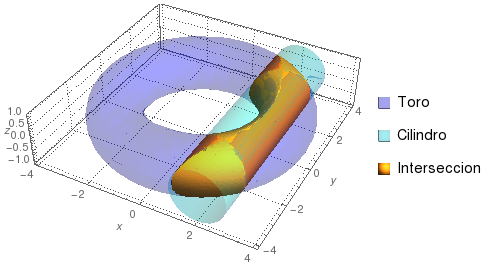
\includegraphics[scale = 0.5]{images/interseccion_P1.png}
  \caption{La figura naranja es el sólido en estudio. Está formado por el volumen que se obtiene al intersectar el toro (celeste) con el cilindro (azul) descritos en la Sección \ref{sec:introduccion_P1}. }
  \label{fig:interseccion_P1}
\end{figure}

En este volumen $W$ se usa el método de Monte Carlo, evaluando puntos generados al azar mediante una distribución uniforme, acotada por los intervalos correspondientes a cada coordenada. En caso de que un punto caiga fuera del sólido, se define $\rho = 0$ para anular su contribución a la integral.

\subsection{Resultados}

Realizando el cálculo con $N = 10^6$ se obtienen los valores de la Tabla \ref{tab:resultados}. Al comparar con la Figura \ref{fig:interseccion_P1} se observa que las coordenadas calculadas para el centro de masa están en el espacio ocupado por el sólido y parecen razonables.

\begin{table}[hl]
\centering
\begin{tabular}{|c|c|c|}
\hline
  Parámetro & Resultado \\
  \hline
  $M$ & $71.00 \pm 0.08$  \\ \hline
  $x_{CM}$ & $2.081 \pm 0.003$\\ \hline
  $y_{CM}$ & $0.001 \pm 0.003$\\ \hline
  $z_{CM}$ & $1 \cdot 10^{-4} \pm 7 \cdot 10^{-4}$\\ \hline
\end{tabular}
\caption{Tabla con resultados del cálculo numérico para la masa $M$ y las coordenadas del centro de masa $x^i_{CM}$.}
\label{tab:resultados}
\end{table}

\subsection{Conclusiones}

En esta ocasión la principal ventaja del método de Monte Carlo ha sido su fácil implementación. Bastó conocer las ecuaciones que acotaban el volumen de integración para poder realizar integración de funciones dentro de él, en este caso de densidad.

Como el algoritmo usado requiere una elevada cantidad de muestras para entregar resultados fiables (en este caso se usaron $10^6$ muestras), hay que tener especial cuidado en acotar lo máximo posible el volumen de pruebas o usar técnicas de optimización para limitar el tiempo de cómputo, que parece ser su principal limitante.

\section{Algoritmo de Metrópolis}

El Algoritmo de Metrópolis

\end{document}
